\section{Mathematical formulation}
\label{section:mathematical model}

In this section, we provide a problem description and describe the stochastic processes and a mathematical model for the seasonal hydropower planning problem.

\subsection{Problem description}
\label{section: problem description}
We consider the medium-term reservoir management problem, where the objective is to value-maximize production over one to two years. The production decisions for medium-term reservoir management are typically of a weekly granularity.  Modern hydropower plants commonly consist of multiple interconnected reservoirs, that allow for coordinated water release that maximizes profit for the system as a whole. The state of the system at a given time is given by the amount of water that is stored in the different reservoirs. Furthermore, as regulations can put constraints on the water stored on a seasonal basis, these constraints can vary for different times $t$.

Several simplifications and assumptions are often made when modelling the reservoir management problem. This includes ignoring operating costs, as these variable costs are usually negligible compared to the revenue. This makes the problem a revenue-maximizing one. Another common simplification is to make the energy coefficient constant, to keep the problem convex. This coefficient is the factor that gives how much energy a production facility can get from a single unit of water. In reality, this factor is dependent on the head (the height difference between the turbine and the variable water level), as well as the intensity of the flow through the turbine. The head can vary substantially with the amount of water in the reservoir. In the sample system, the variations represented between 4.0\% and 6.5\% of the overall head for the different reservoirs, but these variations can be substantially higher or lower depending on the system. Since potential energy increases linearly with the head, this incentivizes producers to keep their reservoir levels high, thereby generating more electricity per unit of water. This poses an interesting dynamic, as the risk of spillage increases with higher water levels. To capture this dynamic, head variations are implemented in the model with a variable energy coefficient. This leads to bi-linearity which is accounted for using McCormick envelopes, similarly to \cite{cerisola2012a}.

\subsection*{Marginal water values}
The main goal of the medium-term reservoir management problem is to estimate marginal water values. These values naturally depend on the amount of water in the system. To illustrate this one can compare the additional value of an extra unit of water in a full reservoir and an empty reservoir. In the case of a full reservoir, one would have to discharge the unit immediately, independently of price, to avoid spillage. If the full reservoir is already producing at full capacity, the additional unit would naturally be spilled, and the marginal value would be 0. For the other extreme case where the reservoir is empty, the marginal value would be much higher as the producer could wait until the prices are high to discharge the unit, without having to worry about spillage. In practice, that means that the marginal value of water decreases, as the water level in the reservoir increases. 

The marginal water value represents the current alternative cost of discharging a unit and is therefore used to make short-term production decisions. The way the medium-term reservoir management problem relates to this is that one can calculate the expected discounted revenue over a 1-2 year horizon starting with different  water levels.  If one plots the expected revenue against the starting water level, the slope of the curve would represent the current marginal water value for different water levels. 

\textcolor{red}{Note that this implies that the main objective of the medium-term reservoir management problem is to estimate the future value function, and, therefore, finding an implementable policy may not be necessary. As a result, the requirement that the optimization method must yield an implementable policy can be relaxed while still making the method useful for supporting short-term decision making.} 


\subsection{Nomenclature}
Before formally defining the optimization model, we provide the notation used for the model in the following section. Some of the notation is only used for the additional constraints seen in the appendix. 
\label{section:notation}
\subsection*{Sets and Indices}
\resizebox{\linewidth}{!}{%
\begin{tabular}{l l}
    
    $R$ & -\hspace{5mm} Reservoirs, indexed by $i$ and $j$ \\\\
    $R^P$ & -\hspace{5mm} Reservoirs with electricity production \\\\
    $R^{Dis}_i$ & -\hspace{5mm} Upstream reservoirs releasing water into reservoir $i$ \\\\
    $R^{Spill}_i$ & -\hspace{5mm} Upstream reservoirs spilling water into reservoir $i$ \\\\
    $\textcolor{red}{M_{i}}$ & -\hspace{5mm} Set of points on the piece-wise linear curve representing the relation between\\
    &\hspace{8.5mm}head and water level for reservoir with electricity production $i$ , indexed by $k$ \\\\
    $\Pi$   & -\hspace{5mm} Set of feasible policies \\\\
    \color{red}
    $\mathcal{S}$   &\color{red} -\hspace{5mm} Set of level 1 scenarios, indexed by $s$ \\\\
    \color{red} $\mathcal{N}$   &\color{red} -\hspace{5mm} Set of level 2 scenarios, indexed by $n$ \\\\
    \color{red} $\mathcal{T}_t$   &\color{red} -\hspace{5mm} Set of stages from stage $t$ to and including the end of the horizon,  indexed by $\tau$ \\\\
\end{tabular}}

\subsection*{Decision Variables}
\begin{tabular}{l l l}
    

    $x_{i,t}$   & -\hspace{5mm} Discharge from reservoir $i$ in period $t$  & [$m^3$] \\\\
    
    $r_{i,t}$   & -\hspace{5mm} Slack variable for water spillage from reservoir $i$ in period $t$  & [$m^3$] \\\\
               
    
    $l_{i,t}$   & -\hspace{5mm} Water level in reservoir $i$ at the beginning of time period $t$ & [$m^3$] \\\\
    
    $l^{avg}_{i,t}$ & -\hspace{5mm} Average water level in reservoir $i$ through time period $t$ & [$m^3$] \\\\
    
    $h_{i,t}$   & -\hspace{5mm} Water head of reservoir $i$ in period $t$     & [$m$] \\\\
    
    $w_{i,t}$   & -\hspace{5mm} Substitution variable for the bi-linear term $h_{i,t}x_{i,t}$ & [$m$] \\\\
    
    $\lambda_{i,t,\textcolor{red}{k}}$ & -\hspace{5mm} Weight of point $k$ on the piece-wise linear graph & \\ 
                & \hspace{6.5mm} describing the relation between  water level       & \\
                & \hspace{6.5mm} and head in reservoir $i$ at time $t$              & \\\\ 
                
   

\end{tabular}

\subsection*{Parameters}
\begin{tabular*}{\textwidth}{@{\extracolsep{\fill}} *{3}{l}   }
    
    $T$        & -\hspace{5mm} Stages (time periods) in planning horizon           & \\\\
    \color{red}
    $S$        & -\hspace{5mm} number of level 1 (outer) scenarios                 & \\\\
    \color{red}
    $N$        & -\hspace{5mm} number of level 2 (inner) scenarios                 & \\\\
    \color{black}
    $\beta$     & -\hspace{5mm} Discount factor                                     & \\\\
    
    $\eta_{i}$  & -\hspace{5mm} constant factor describing the efficiency of the    & [$MWh/m^3$] \\
                & \hspace{6.5mm}  turbine of  reservoir $i$                         & \\\\
    
    $g$      & -\hspace{5mm} gravitational acceleration constant &[$m/s^2$] \\\\
    
    $\rho$      & -\hspace{5mm} density of water &[$Kg/m^3$] \\\\

    $P_{t}$     & -\hspace{5mm} Power price in stage $t$                            & [\euro$/MWh$] \\\\
    
    $I_{i,t}$   & -\hspace{5mm} Water inflow intensity for reservoir $i$ in period $t$ & [$m^3$] \\\\
    
    %$L_{i}^{0}$ & -\hspace{5mm} Initial water level for reservoir $i$               & [$m^3$] \\\\
    %$H_{i,t}^{max}, H_{i,t}^{min}$ & -\hspace{5mm} Maximum and minimum water head level in reservoir $i$ in period $t$ & [$m$] \\\\

\end{tabular*}





\subsection{Stochastic processes}
\textcolor{red}{Restructured energy markets have uncertain prices, denoted $P_t$, which means that modellers have to optimize over stochastic prices.} Furthermore, as weather cannot be forecasted perfectly, the inflow to reservoirs is also uncertain. The set of all reservoirs is denoted by $R=\{1,2,...,|R|\}$. We denote inflow to reservoir $i \in R$ at time $t$ by $I_{i,t}$.

For prices, we apply the Schwartz-Smith two-factor model \cite{schwartz2000a}. This model assumes that the logarithm of the price can be modelled as the sum of a short-term factor, a long-term factor, and finally a seasonal factor, as the energy price typically follows a seasonal pattern. The model parameters are estimated using Kalman filtering and maximum likelihood estimation \cite{goodwin2013a}. Data points are obtained from synthetic futures curves \cite{dietze} using the approach in \cite{benth2007a}.

The inflow model is primarily based on the one seen in \cite{gjelsvik2010a}, where the inflow is modelled according to AR-1 processes. To reduce dimensionality and capture the covariance of inflow to different reservoirs, a PCA transformation of the inflow data is performed to project it to a lower dimensionality, as seen in \cite{da_Costa2006}. The original inflow data is normalized to follow a standard normal distribution, before being transformed using PCA. After fitting AR-1 models to the lower dimension data, one can produce scenarios using the model for every dimension $k$ in the projected space. After generating the low-dimensional scenarios, we can transform the generated scenario back to the original dimensionality, using the PCA matrix. We then denormalize this data, to ensure that the generated scenarios follow the distribution of the historical observations. To circumvent the issue of negative inflows generated by the AR model, negative values are converted to 0 according to equation \eqref{eq:force_positive}. 


\begin{equation}
\label{eq:force_positive}
   I_{i,t} = \max(I_{i,t},0)
\end{equation}

\subsection{Actions and transition function}
We present here stage-$t$ actions and transition functions. As only a subset of these reservoirs have connected turbines allowing for energy production, we denote this by subset $R^P = \{1,2,...,|R^P|\}$. These sets are both indexed by $i$ and $j$, for the modelling of interconnections between reservoirs. Every reservoir $i$, have two sets of reservoirs $R^{Dis}_i$ and $R^{Spill}_i$, \textcolor{red}{that respectively represent the reservoirs whose discharged and spilled water flows directly into reservoir $i$}.

The vector of decisions in stage $t$ includes discharge $x_{i,t}$ and spillage $r_{i,t}$ for each station and reservoir, where $\Pi_t(l_t,I_t)$ is the feasible stage-$t$ action set and $(x_{i,t},r_{i,t}, \ i \in R) \in \Pi_t(l_t,I_t)$. The discharge variable has both upper and lower bounds depending on physical limitations and regulations that can be seasonal. The spillage and the discharge can naturally not be negative. %The action set $A_t(l_t,m_t)$ is given in the Appendix.

The transition function consists of three components $(l_t,P_t,I_t)$. The exogenous components, includes price $P_t$ and the vector of inflows, $I_t = (I_{i,t}, \ i \in R)$. These factors get updated according to the stochastic processes discussed in the previous section, independently of the stage-$t$ action. The endogenous component is the vector of reservoir volumes in the watercourse, $l_t = (l_{i,t}, \ i \in R)$. Executing an action $(x_t,r_t)$ at stage $t$ and state $(l_t,P_t,I_t)$ leads to the following update of the endogenous state,
\begin{equation}
\label{eq:inventory_balance}
    l_{i,t+1} = l_{i,t} + I_{i,t} - r_{i,t} - x_{i,t} + \sum_{j\in R_{i}^{Spill}} r_{j,t}+ \sum_{j\in R_{i}^{Dis}} x_{j,t},\\ \quad  i\in R. % \quad t=0,..,T-1
\end{equation}
This function ensures \textcolor{red}{water} balance in time and the topology of the watercourse. It gives the relationship between the inflow, production decisions, spillage, and the water level of a given reservoir $i$. It ensures that spillage happens when the net inflow is higher than the reservoir capacity. Due to the longer time steps taken with medium-term reservoir management, water delay is not taken into account, and it is assumed that water can flow through the entire system within a single time step. 



\subsection{Immediate reward and policy}
At each stage, the immediate reward is given by electricity production and electricity price (\ref{eq:reward})
\begin{equation}
    P_{t}\sum_{i\in R^P}g(l_{i,t},x_{i,t}),
    \label{eq:reward}
\end{equation}
where $g(l_{i,t},x_{i,t})$ is the energy output from discharge $x_{i,t}$ at reservoir level $l_{i,t}$. We denote the set of feasible policies by $\Pi$. A policy $\pi$ is a collection of stage-dependent actions, mapping states at time $t$ to feasible actions. We let $l_{i,t}^{\pi}$ and $x_{i,t}^{\pi}$ respectively denote the endogenous state reached at, and action made in, stage $t$ for reservoir $i$, when following policy $\pi$. We aim to find a policy that maximizes the expected accumulated discounted reward,
\begin{equation}
\label{eq:objective_function_bilinear}
\begin{split}
    V_0(l_0, \textcolor{red}{I_0,P_0}) =  \max_{\pi \in \Pi} \mathbb{E}\left[\textcolor{red}{\sum_{t=0}^{T-1}}\beta^{t}P_{t}\sum_{i\in R^P}g(l^{\pi}_{i,t},x^{\pi}_{i,t}) + \beta^{T}\sum_{i\in R}\Phi_{i}(l^{\pi}_{i,T})\bigg|\textcolor{red}{I_0,P_0}\right],
\end{split}
\end{equation}
where $\beta$ is the discount factor and $\Phi(l_{i,T})$ is the end of horizon value for each reservoir, given by how much water is remaining.

\subsection{Relaxation and approximations}
The reward function contains the term $g(l_{i,t},x_{i,t})$. This function is typically concave in $l_{i,t}$ and $x_{i,t}$. The higher the reservoir, the higher the generation output. Similarly, as a function of discharge, the efficiency of a turbine is first increasing and then possibly decreasing. Piece-wise linear approximations of the discharge function can handle the latter feature. In our model, we assume it to be a constant factor for each reservoir $i$ denoted $\eta_{i} \in[0,1]$, i.e.\ $g(l_{i,t},x_{i,t})=g(l_{i,t})x_{i,t}\eta_i$. The dependency of reservoir volume, i.e.\ head variations, is complicated since it leads to a bi-linear objective and thereby non-convexity. This makes it challenging to optimize with conventional methods such as SDDP, which we use as a baseline. To deal with this issue, we relax the problem using McCormick envelopes. We start by modifying the reward in \eqref{eq:reward} to 

\begin{equation}
    P_{t}\sum_{i\in R^P} h_{i}(l_{i,t})x_{i,t}g\rho\eta_i
    \label{eq:reward2}
\end{equation}
The functions $h_{i}(\cdot)$ represent the head in reservoir $i$, while $g$ is the gravitational acceleration constant and $\rho$ is the density of water. The $h_{i}(\cdot)$ functions depend on $l_{i,t}$ and are calculated using piece-wise linear approximations for the individual reservoirs. \textcolor{red}{These piece-wise linear graphs are represented as sets of points, where the x-coordinate represents the water level and the y-coordinate represents the head. These sets are denoted $M_i$, for every reservoir $i$.  To find the head $h_{i,t}$ given any feasible water level $l_{i,t}$, we introduce the variables $\lambda_{i,t,k}$ representing the weight of every point $k \in M_i$ at time $t$. By ensuring that all these weights are non-negative and sum to 1, and that at most two points adjacent to each other can be non-zero, we can find the exact point on the y-axis on the piece-wise linear graph, given the value on the x-axis.} 

The restriction requiring that at most two weights can be non-zero, and that these must represent points adjacent to each other, is called a special ordered set of type 2 (SOS2) restriction. This restriction can be ignored in cases where the piece-wise linear function is concave, as the head $h_{i,t}$ would be the same with or without the SOS2 constraint. The approximated graphs for the energy-producing reservoirs in the Matre Haugsdal system can be seen in Figure \ref{fig:head_res_relations_Matre_H}. It can be seen that these are all concave, ensuring that the SOS2 constraints are unnecessary. 


\begin{figure}[h]
     \centering
          \begin{subfigure}[b]{0.25\textwidth}
         \centering
         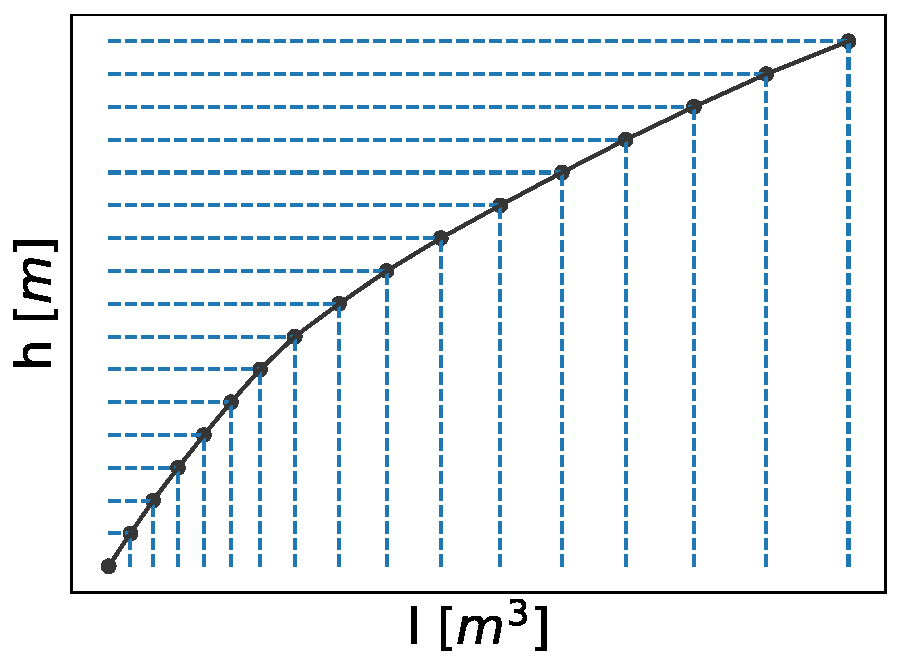
\includegraphics[width=\textwidth]{head_res_relation_Svartevatn1.pdf}
         \caption{Svartevatn}
         \label{fig:head_res_relation_Svartevatn}
     \end{subfigure}
     \hfill
     \begin{subfigure}[b]{0.25\textwidth}
         \centering
         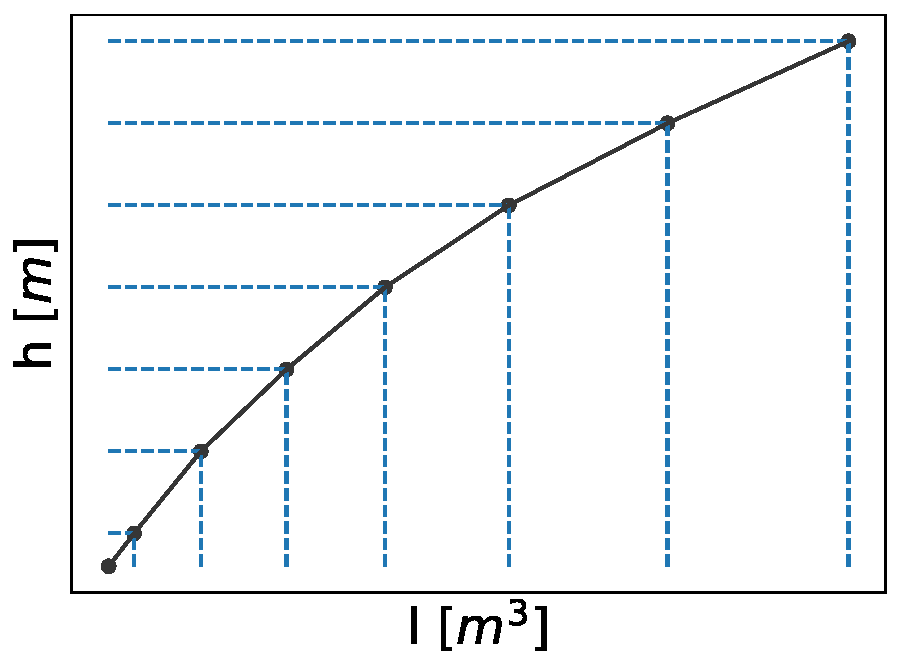
\includegraphics[width=\textwidth]{head_res_relation_Storevatn1.pdf}
         \caption{Storevatn}
         \label{fig:head_res_relation_Storevatn}
     \end{subfigure}
     \hfill
     \begin{subfigure}[b]{0.25\textwidth}
         \centering
         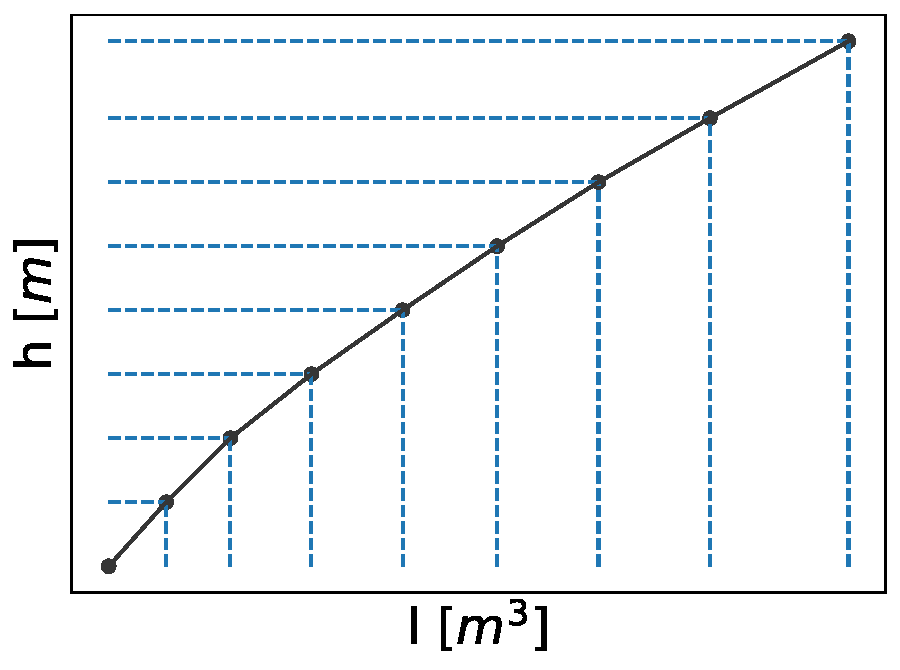
\includegraphics[width=\textwidth]{head_res_relation_Gobotvatn1.pdf}
         \caption{Gobotvatn}
         \label{fig:head_res_relation_Gobotvatn}
     \end{subfigure}
        \caption{Volume-head relations for reservoirs with production}
        \label{fig:head_res_relations_Matre_H}
\end{figure}



The piece-wise linear approximation of the head function $h_{i}(l_{i,t})$ is explained in further detail in Appendix \ref{appendix: Piece-wise linear}. This approximation leads to bi-linear terms in \eqref{eq:reward2}. To approximate these terms, we introduce the substitution variable $w_{i,t}=h_{i}(l_{i,t})x_{i,t}$ and use McCormick envelope constraints. This gives us the modified linear reward
\begin{equation}
    P_{t}\sum_{i\in R^P} w_{i,t}g\rho\eta_i,
    \label{eq:reward3}
\end{equation}
which leads to a convex and linear multistage optimization problem, satisfying the requirements of SDDP. For additional constraints associated with the McCormick relaxation, see Appendix \ref{Appendix: McCormick constraints}.

